\chapter{Auswahl und Bewertung der Hard- und Softwarekomponenten}

\section{Hardwarekomponenten}

\subsection{Mikrofonmodule}

Zur Erfassung des Lautstärkepegels wurden drei unterschiedliche Mikrofonmodule in Betracht gezogen. 
Der erste Sensor ist ein kostengünstiges Modul "GY-MAX4466" (ca.\ 4\,€), das ursprünglich als Klatschsensor konzipiert wurde. 
Der zweite Sensor ist das \textit{Sound Level Meter V2.0} von DFRobot (ca.\ 40\,€), das über zusätzliche Hardware zur Signalverarbeitung verfügt und den Schalldruckpegel bereits gefiltert und bereinigt im dBA-Format ausgibt.
Der dritte in Betracht gezogene Sensor ist ein handelsübliches DB-Messgerät (ca.\ 20\,€), das jedoch nicht für die Integration in das Projekt geeignet ist, da es keine digitale Schnittstelle bietet und somit nicht direkt mit dem ESP32 kommunizieren kann.
Dieser Sensor wird daher zur Überprüfung der Ergebnisse verwendet, ist aber nicht für die direkte Integration in das Projekt vorgesehen.

Da die absolute Einheit (dBA) für die Auswertung im Rahmen eines 3D-Diagramms nicht zwingend erforderlich ist, wurde der Fokus auf die Vergleichbarkeit der analogen Ausgangssignale gelegt. 
Beide Sensoren wurden gleichzeitig an einem ESP32 betrieben und ihre Ausgangssignale mithilfe des \textit{Serial Plotter} in Echtzeit visualisiert. 
Dabei zeigte sich, dass die Kurvenverläufe bei normalen Sprachgeräuschen nahezu identisch sind. 
Lediglich bei impulsartigen Geräuschen mit sehr geringer Distanz (z.\,B.\ Klatschen oder Klopfen) erzeugt das günstigere Mikrofon deutlich stärkere Peaks, während diese durch den DFRobot-Sensor wirksam herausgefiltert werden.

\begin{center}
  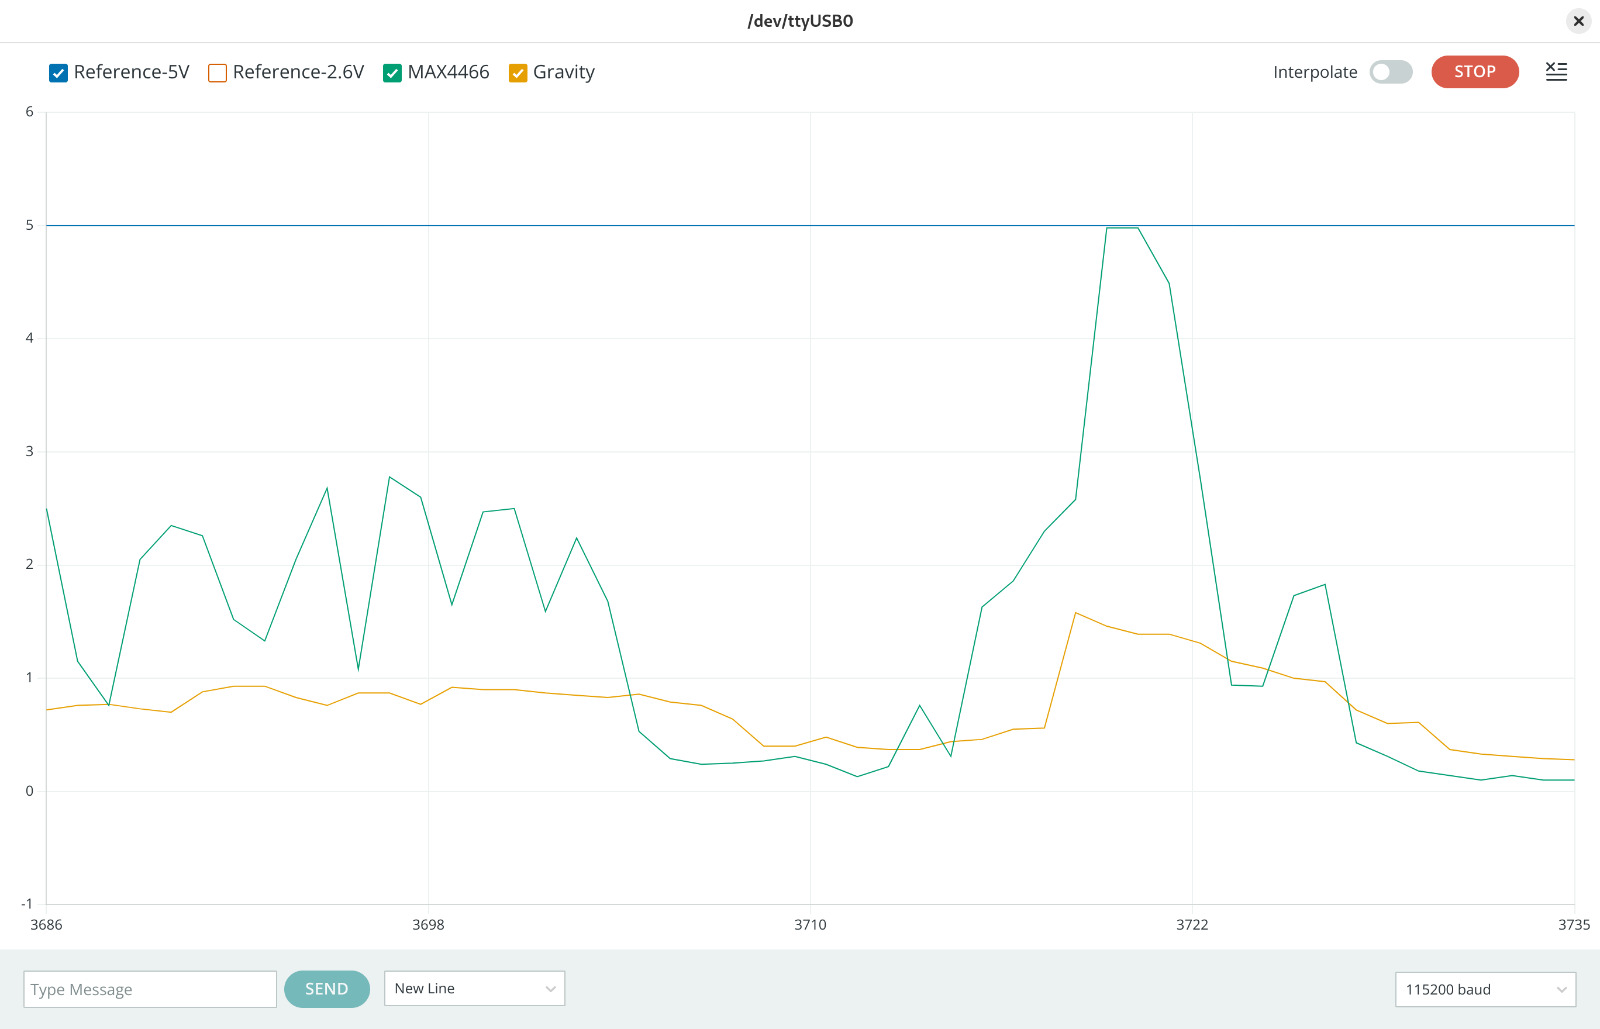
\includegraphics[width=1\textwidth]{../images/Sensorvergleich/PeekSensorVergleich.jpeg}
\end{center}
\begin{center}
  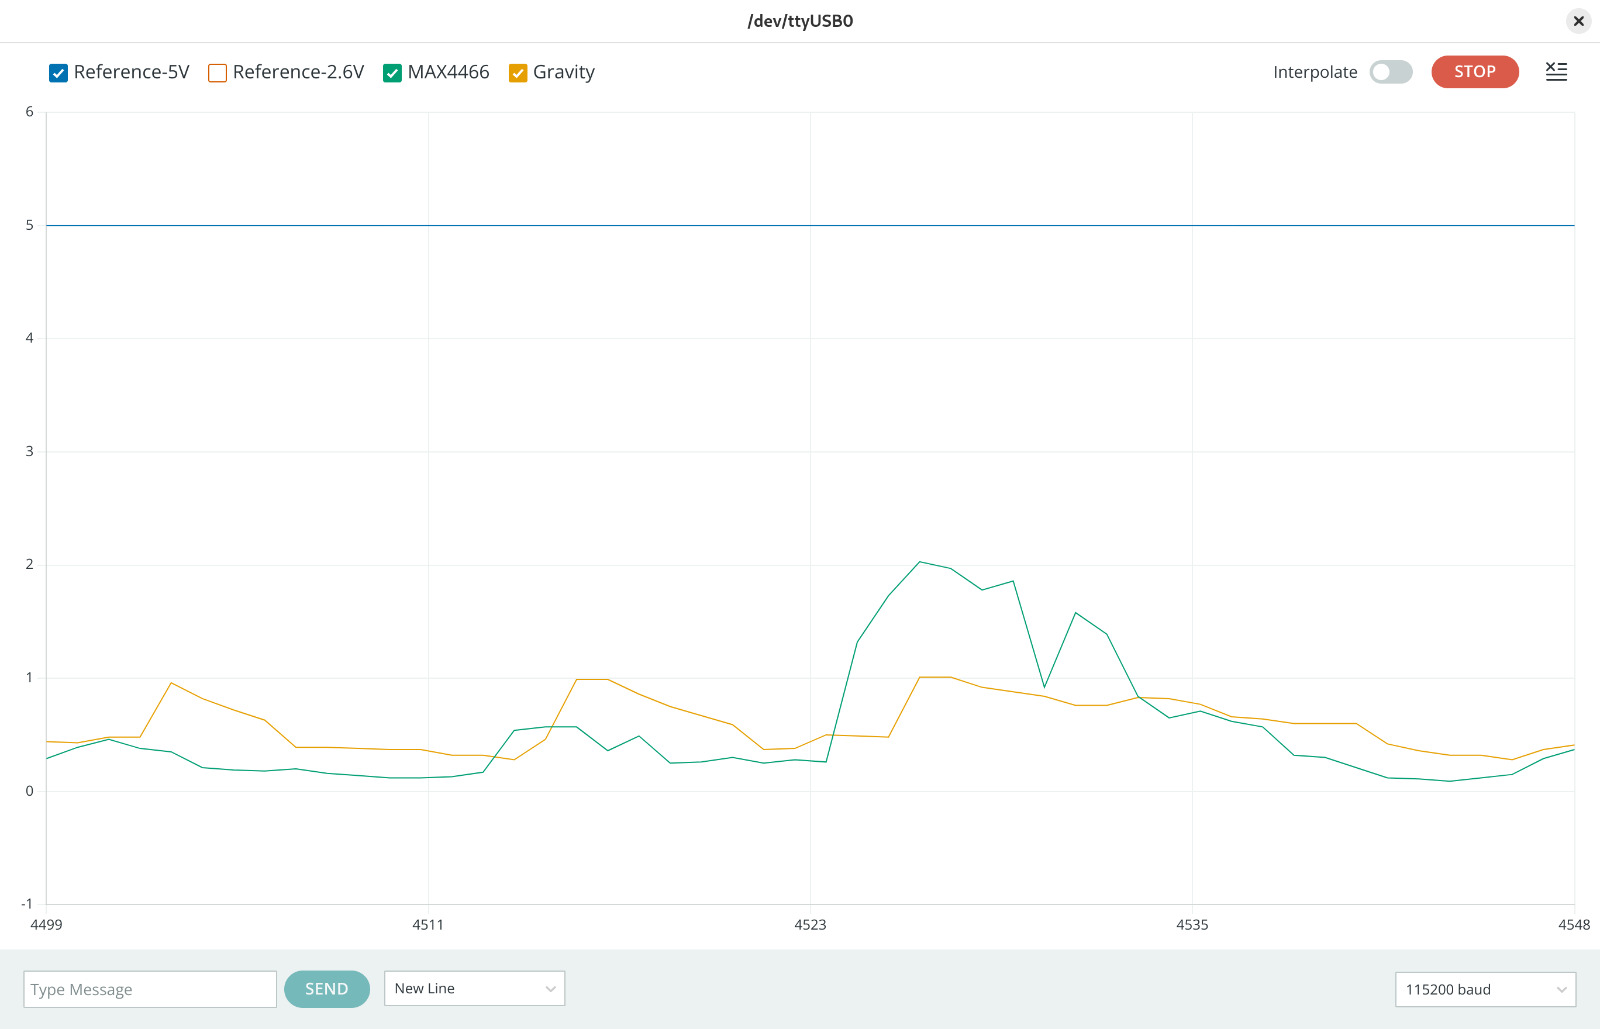
\includegraphics[width=1\textwidth]{../images/Sensorvergleich/StaticSensorVergleich.jpeg}
\end{center}

Hier sind die Sensorwerte des günstigeren Klatschsensors (grün), sowie die des Teureren Dba sensors (gelb) dargestellt. Die In Blau dargestellte 5v Referenzlinie stellt den Maximalwert da, welcher von den Sensoren zurückgegeben werden kann.

Da die in den Vergleichsdiagrammen dargestellten Abweichungen bei größerem Abstand deutlich abnehmen und im Anwendungsfall als vernachlässigbar eingestuft werden können, wurde entschieden, den günstigeren Sensor zu verwenden. 
Um mögliche Reststörungen dennoch weiter zu reduzieren, ist geplant, eine mechanische Dämpfung oder Abschirmung am Sensor zu testen.

Insgesamt konnte festgestellt werden, dass der günstigere Sensor trotz fehlender dBA-Ausgabe für die angestrebte Visualisierung ausreichend präzise Ergebnisse liefert und somit für den weiteren Projektverlauf verwendet wird.

\section{Softwarekomponenten}
\subsection{Entwicklungsumgebungen}

Zu Beginn des Projekts wurden zwei gängige Entwicklungsumgebungen für die Programmierung von Mikrocontrollern evaluiert: die klassische \textit{Arduino IDE}, welche auch von den betreuenden Dozierenden empfohlen wurde, sowie die moderne, zunehmend verbreitete \textit{PlatformIO}-Erweiterung für Visual Studio Code.

Im Projektteam wird plattformübergreifend mit Linux, Windows 10 und Windows 11 gearbeitet. Beide Entwicklungsumgebungen sind grundsätzlich mit allen eingesetzten Betriebssystemen kompatibel. Zur Prüfung der technischen Umsetzbarkeit wurden zwei separate Repositories eingerichtet, in denen jeweils einfache Testprojekte zur Ansteuerung eines ESP32 implementiert wurden.

Beide IDEs konnten den Mikrocontroller erfolgreich ansprechen. PlatformIO bietet durch seine deklarative Verwaltung von Bibliotheken und Abhängigkeiten Vorteile in Bezug auf Reproduzierbarkeit und Build-Konsistenz. In der Praxis kam es jedoch auf einem System im Team zu anhaltenden technischen Problemen mit PlatformIO, die nicht zufriedenstellend gelöst werden konnten.

Um eine einheitliche und zuverlässige Entwicklungsgrundlage für alle Teammitglieder sicherzustellen, fiel die Entscheidung letztlich zugunsten der \textit{Arduino IDE}. Diese ermöglicht eine barrierefreie Mitarbeit aller Beteiligten, auch wenn sie im Funktionsumfang nicht ganz an PlatformIO heranreicht.

\subsection{Kommunikationsmethode}
ESP-NOW wurde ausgewählt, da es im Vergleich zu anderen Protokollen einen deutlich geringeren Overhead besitzt und dadurch eine schnellere und effizientere Datenübertragung ermöglicht. Die Struktur ist weniger komplex, was die Implementierung vereinfacht und die Fehleranfälligkeit reduziert. 
Dadurch wird das System insgesamt robuster und zuverlässiger:
ESP-Now ist ein Kommunikationsprotokoll von Espressif, das speziell für die ESP32- und ESP8266-Chips entwickelt wurde. Es verwendet die 2,4 Ghz Frequenz, welche eigentlich für WiFi Kommunikation verwendet wird. 
Im Gegensatz zu anderen Protokollen sind die Nachrichten auf Schicht 2 des ISO-OSI-Modells. Keine IP-Adressen sondern nur MAC-Adressen. Die ESPs müssen sich dafür im gleichen Kanal befinden. Die 2,4 Ghz Frequenz hat grundsätzlich nur 3 Nutzbare Kanäle. 
Der zu verwendene Kanal muss von dem "AI401" Wlan Netz übernommen werden.Es ist mit relativ wenig Code möglich eine große Menge an Daten in sehr Kurzen Zeitabschnitten zu senden. Theoretisch ist eine Datenübertragung von 1 bis 2 Mbps möglich. 
Die Nachrichtenlänge ist auf 250 Byte pro Paket beschränkt. Da unsere Nachrichten nur wenige Bit lang sind, haben wir hier keine Probleme. 
Das Protokoll hat keine festgelegten Sender/Empfänger Rollen. Jeder ESP kann senden und empfangen. In unserem Beispiel senden aber 3 ESPs und ein Edge-Device empfängt alle Daten. 
Es wird 10 mal pro Sekunde der Lautstärkepegel erfasst und gesendet.

\subsection{ESP32}
Die ESP-Module bieten im Vergleich zu klassischen Arduinos eine integrierte WLAN-Funktionalität und unterstützen direkt das ESP-NOW-Protokoll. Dadurch entfällt zusätzlicher Hardware- oder Softwareaufwand für die Netzwerkkommunikation.
In Kombination mit ESP-NOW ergibt sich somit eine kompakte, performante und zuverlässige Lösung.

\subsection{Frontend}
Für die Umsetzung des Frontends wurde Angular gewählt, 
da im Team bereits umfangreiche Erfahrung mit diesem Framework vorhanden war. 
Angular bietet eine klare Struktur durch komponentenbasiertes Design, 
erleichtert die Wiederverwendbarkeit von UI-Elementen und unterstützt eine saubere Trennung von Logik und Darstellung. 
Dadurch konnte effizient und wartbar entwickelt werden.

Das Frontend läuft in einem eigenen Docker-Container und kommuniziert, 
über ein internes Netzwerk, mit dem separat laufenden Backend-Container. 
So bleibt die Architektur modular, skalierbar und einfach wartbar.

Die Darstellung der Daten wird über Angular-Komponenten realisiert,
die Visualisierung in einfachen Liniendiagrammen wird mit der ng2-charts-Bibliothek ermöglicht.
\begin{center}
  \includegraphics[width=1\textwidth]{../images/LinechartFE.png}
\end{center}

\subsection{Backend}
Das Backend wurde mit Node.js und dem minimalistischen Framework Express.js umgesetzt. 
Express ist das am weitesten verbreitete Node.js-Framework für Webserver und APIs. 
Es bietet eine ausgereifte Middleware-Architektur, die sehr flexibel und modular ist. 
Im Vergleich zu ähnlich minimalistischen Frameworks wie Koa, 
das von den gleichen Entwicklern stammt, 
bietet Express mehr out-of-the-box Funktionalitäten und eine größere Community mit umfangreichen Plugins und Support. \cite{betterstack2025koavsexpress,appventurez2025nodejsframework}

Koa hingegen ist moderner und basiert stärker auf ES6 Features wie async/await, was den Code oft sauberer macht. 
Allerdings ist Koa weniger „batteries included“ und erfordert mehr Initialaufwand und zusätzliche Libraries, 
um Funktionen bereitzustellen, die Express standardmäßig mitbringt. 
Für dieses Projekt, welches einen schnellen Einstieg, umfangreiche Dokumentation und stabile Middleware braucht, 
ist Express daher die pragmatischere Wahl.
Zudem sind Gruppenmitglieder bereits mit Express vertraut, was die Einarbeitungszeit verkürzt und die Produktivität steigert. 

Die Anbindung an eine InfluxDB erfolgt über die offizielle Client-Bibliothek. Die Entscheidung für InfluxDB basiert auf der Empfehlung der "Verteilten Systeme"-Dozenten sowie der nahtlosen Integration in das Node.js-Backend, was die Implementierung vereinfacht.
Neben dem Abrufen historischer Sensorwerte werden auch Funktionen zum Schreiben von Dummy-Daten bereitgestellt.
Diese werden, solange die Verbindung zu den wirklichen Sensorwerten noch nicht hergestellt ist, zum Testen verwendet.

Das Backend ist ebenfalls in einem eigenen Docker-Container gekapselt. 
Die Kommunikation mit dem Frontend erfolgt über definierte HTTP-Endpunkte im Container-Netzwerk. 
Diese Trennung verbessert die Wartbarkeit und erlaubt eine flexible Skalierung beider Komponenten unabhängig voneinander.
